\chapter{Introducción específica} % Main chapter title

\label{Chapter2}

%----------------------------------------------------------------------------------------
%	SECTION 1
%----------------------------------------------------------------------------------------
En este capítulo se introduce la terminología específica de la red de comunicaciones del tren (TCN) y del sistema de información visual al pasajero (PIDS). La arquitectura del sistema y  sus módulos principales son presentados con una descripción general. Además, se introduce el sistema de carteles led de Trenes Argentinos, que son los que brindan información al pasajero en las formaciones ferroviarias operativas de la empresa.\\


\section{Red de comunicación del tren TCN}

La red de comunicaciones del tren TCN presenta una arquitectura de buses jerárquicos de dos niveles, y está especificada en el estándar IEC-61375-1 \cite{IEC-61375-1999} de la \textit{International Electrotechnical Commission} (IEC). En la figura \ref{fig:redTCN} se presenta el esquema de conexión de los buses de datos de la TCN, el \textit{Wire Train Bus} (WTB) que se encarga de las comunicaciones entre coches a través de nodos con redundancia física, y el \textit{Multi Vehicle Bus} (MVB), al que se conectan los dispositivos de cada coche. 
Cada bus de datos tiene su especificación de detalle en las normas de la IEC \citep{CSN-EN-61375-2-1} y \citep{IEC-61375-3-1:2012}. \\

\begin{figure}[H]
	\centering
	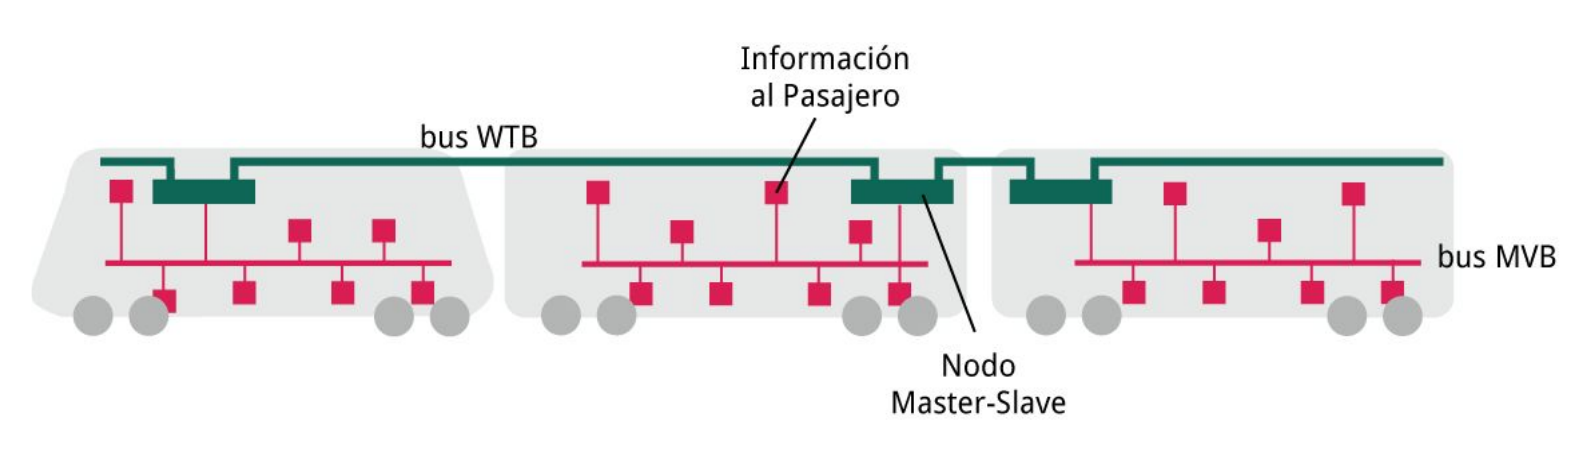
\includegraphics[width=1\textwidth]{./Figures/diagramaRedTCN.png}
	\caption{Diagrama del tren y de los buses WTB/MVB de la red TCN.}
	\label{fig:redTCN}
\end{figure}

En la figura \ref{fig:sofseTCN} se presenta la topología de la red TCN para los trenes de SOFSE. Observar que, leyendo la figura desde arriba hacia abajo, el esquema sugiere la ubicación en los coches de los distintos módulos. En los trenes de SOFSE, existen armarios con racks en los extremos de los coches, donde se alojan los dispositivos de la red.\\ \pagebreak

\begin{figure}[H]
	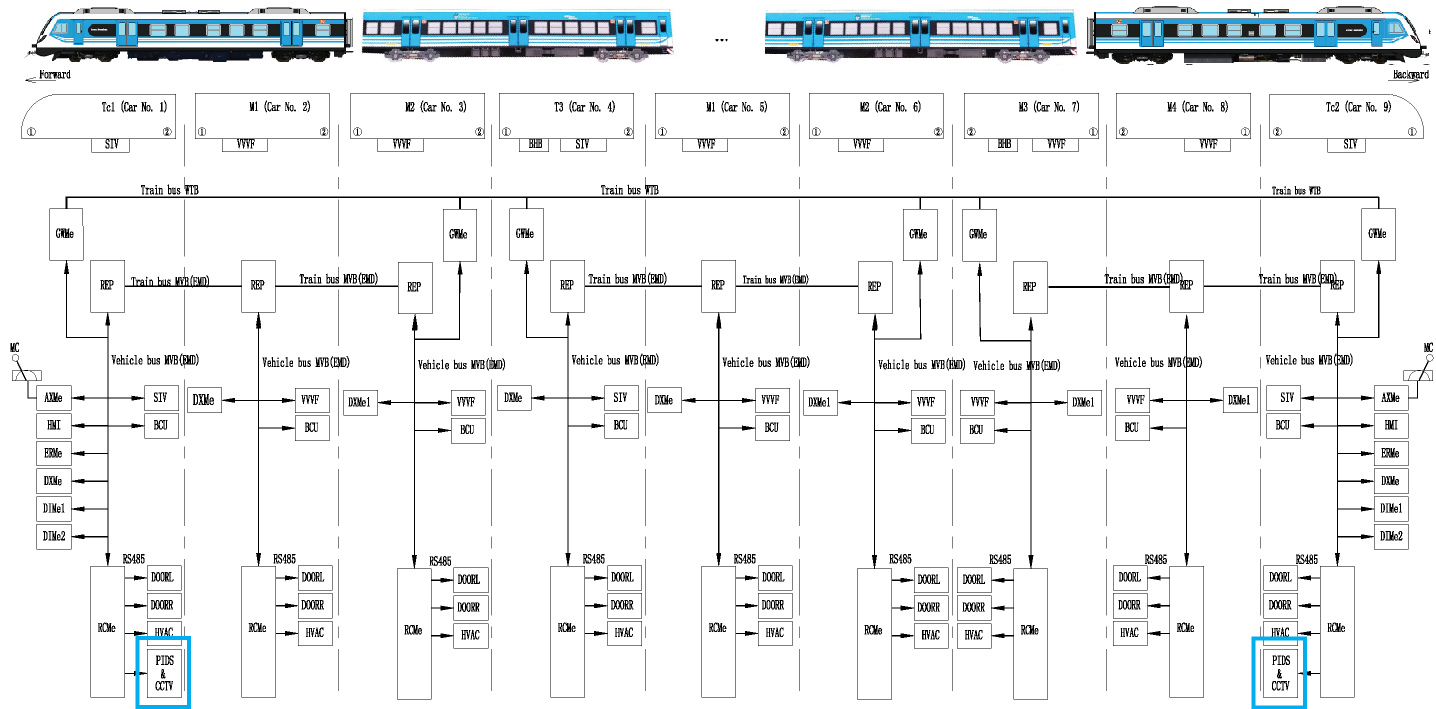
\includegraphics[width=1.8\textwidth, angle=90]{./Figures/diagramaTrenesArgentinosTCN2.png}
	\caption{diagrama de la red TCN de Trenes Argentinos. Plano cortesía SOFSE, editado por el autor.}
	\label{fig:sofseTCN}
\end{figure}


 En la figura \ref{fig:sofseTCN} también se puede observar que varios de los módulos se repiten en cada coche y, resaltado en celeste, se señala la ubicación del sistema PIDS y del circuito cerrado de TV (CCTV) en los coches cabecera. Los buses MVB y WTB también están representados en la topología a lo largo del tren. El nodo \textit{Master-Slave} que interconecta los buses está representado por un bloque denominado GWMe, \textit{Vehicle control module} según la nomenclatura oficial, y funciona de \textit{gateway} entre ambos buses. Siguiendo la cascada de bloques, todos los módulos que le siguen a los bloques REP (\textit{Trunk module}) están conectados al bus MVB. Algunos de los dispositivos y sistemas conectados al MVB que se pueden observar son: el control de puertas (DOORL/R), el aire acondicionado (HVAC), el sistema de tracción (VVVF), el sistema de control de frenos (BCU), entre otros. \\

En las figuras \ref{fig:imgRackTCN} y \ref{fig:rackPIDS1} se presentan fotografías de los armarios de los trenes donde se puede ver la disposición de los equipos en los racks de salón. Los módulos negros que se observan en la figura \ref{fig:imgRackTCN} se denominan DIMe, DXMe y RCMe, y son parte de la solución TCN del Instituto Zhuzhou, denominada Distribute Train Electric Control System (DTECS)  \cite{feng2016survey}. \\

En la parte inferior del rack, se puede observar un bloque de módulos grises señalados como parte del sistema PIDS. El mapa de recorrido led (LMDU), los carteles de matriz led (IDU), los parlantes (LSP) y las cámaras de video (CCTV), son parte del PIDS, que también se interconectan al bus MVB. Acorde a la topología, el PIDS se conecta a un módulo denominado RCMe, a través de una red RS485. Este último bloque se corresponde con el módulo RCMe, recuadrado en celeste en la figura \ref{fig:imgRackTCN}.  Según lo relevado en las formaciones de Trenes Argentinos, y también en el plano de la red TCN, el PIDS tiene su propia red RS485, aparte de la que corresponde a la interconexión con el MVB. La figura \ref{fig:rackPIDS1} es una fotografía en detalle de la unidad de rack donde están instalados los módulos de hardware del PIDS. \\

\begin{figure}[htbp]
	\centering
	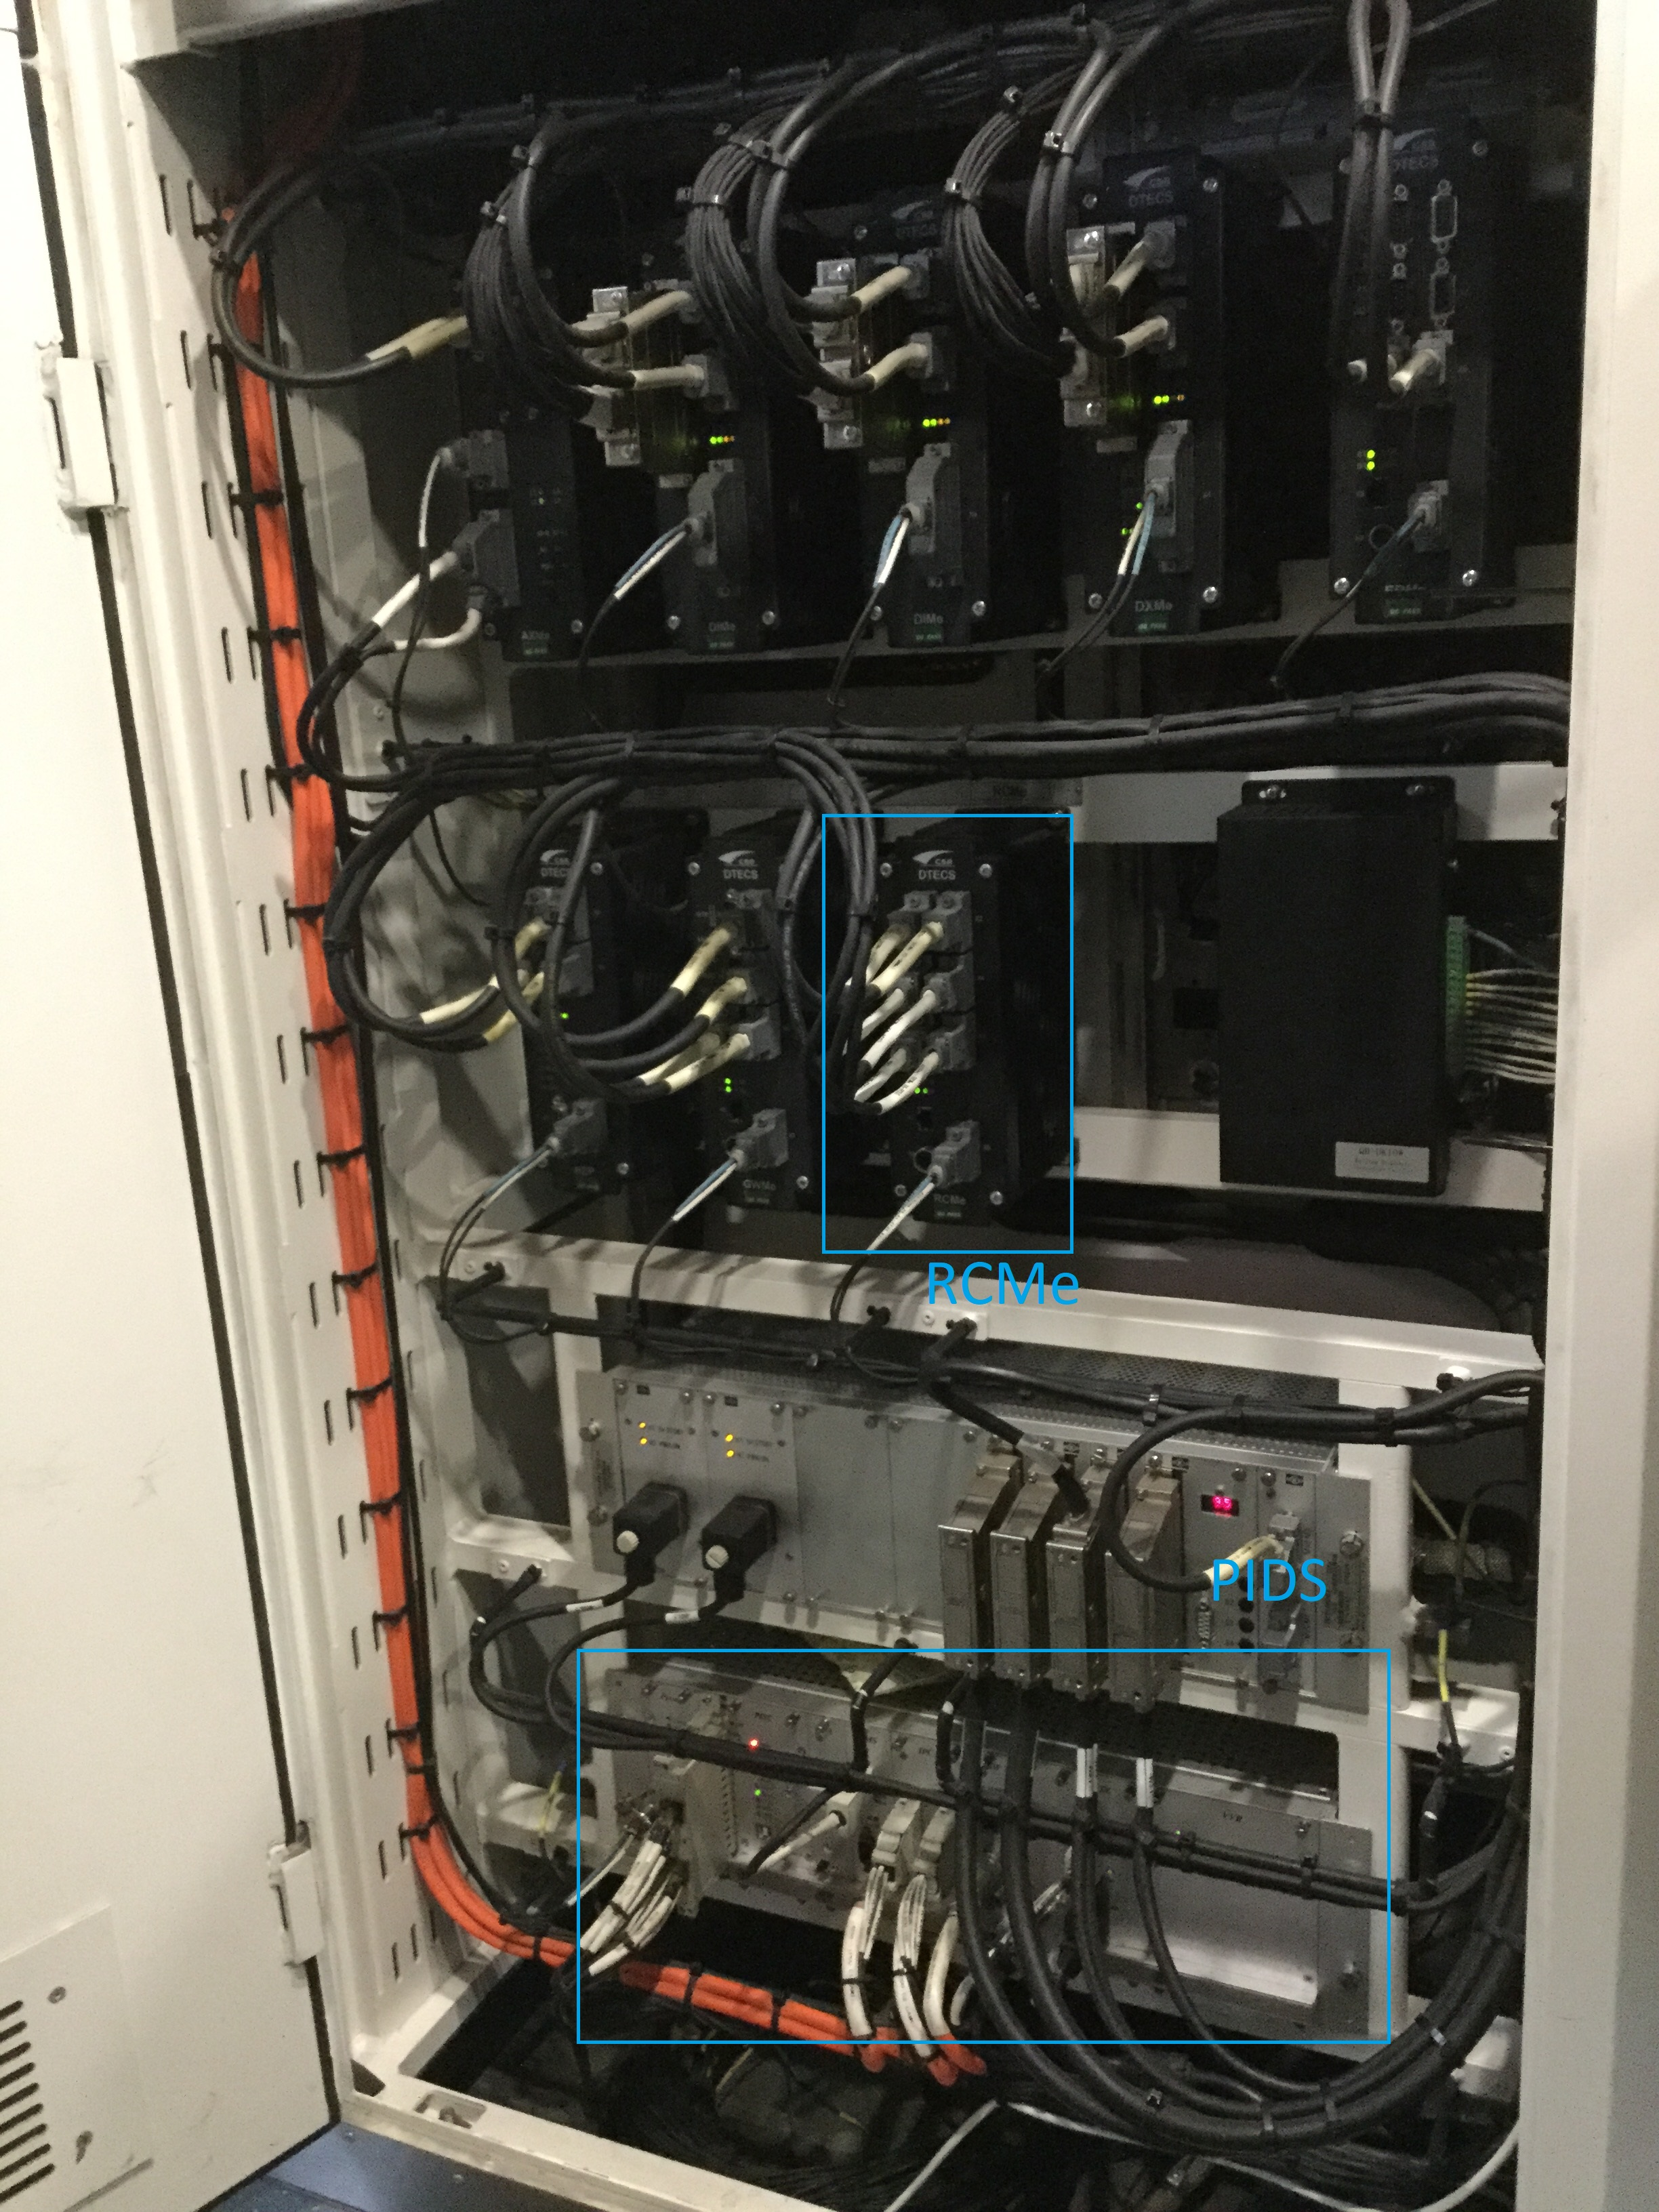
\includegraphics[width=0.75\textwidth , angle=0]{./Figures/imgRackTCN.JPG}
	\caption{Fotografía del rack de salón de una formación de Trenes Argentinos.}
	\label{fig:imgRackTCN}
\end{figure}

\begin{figure}[htbp]
	\centering
	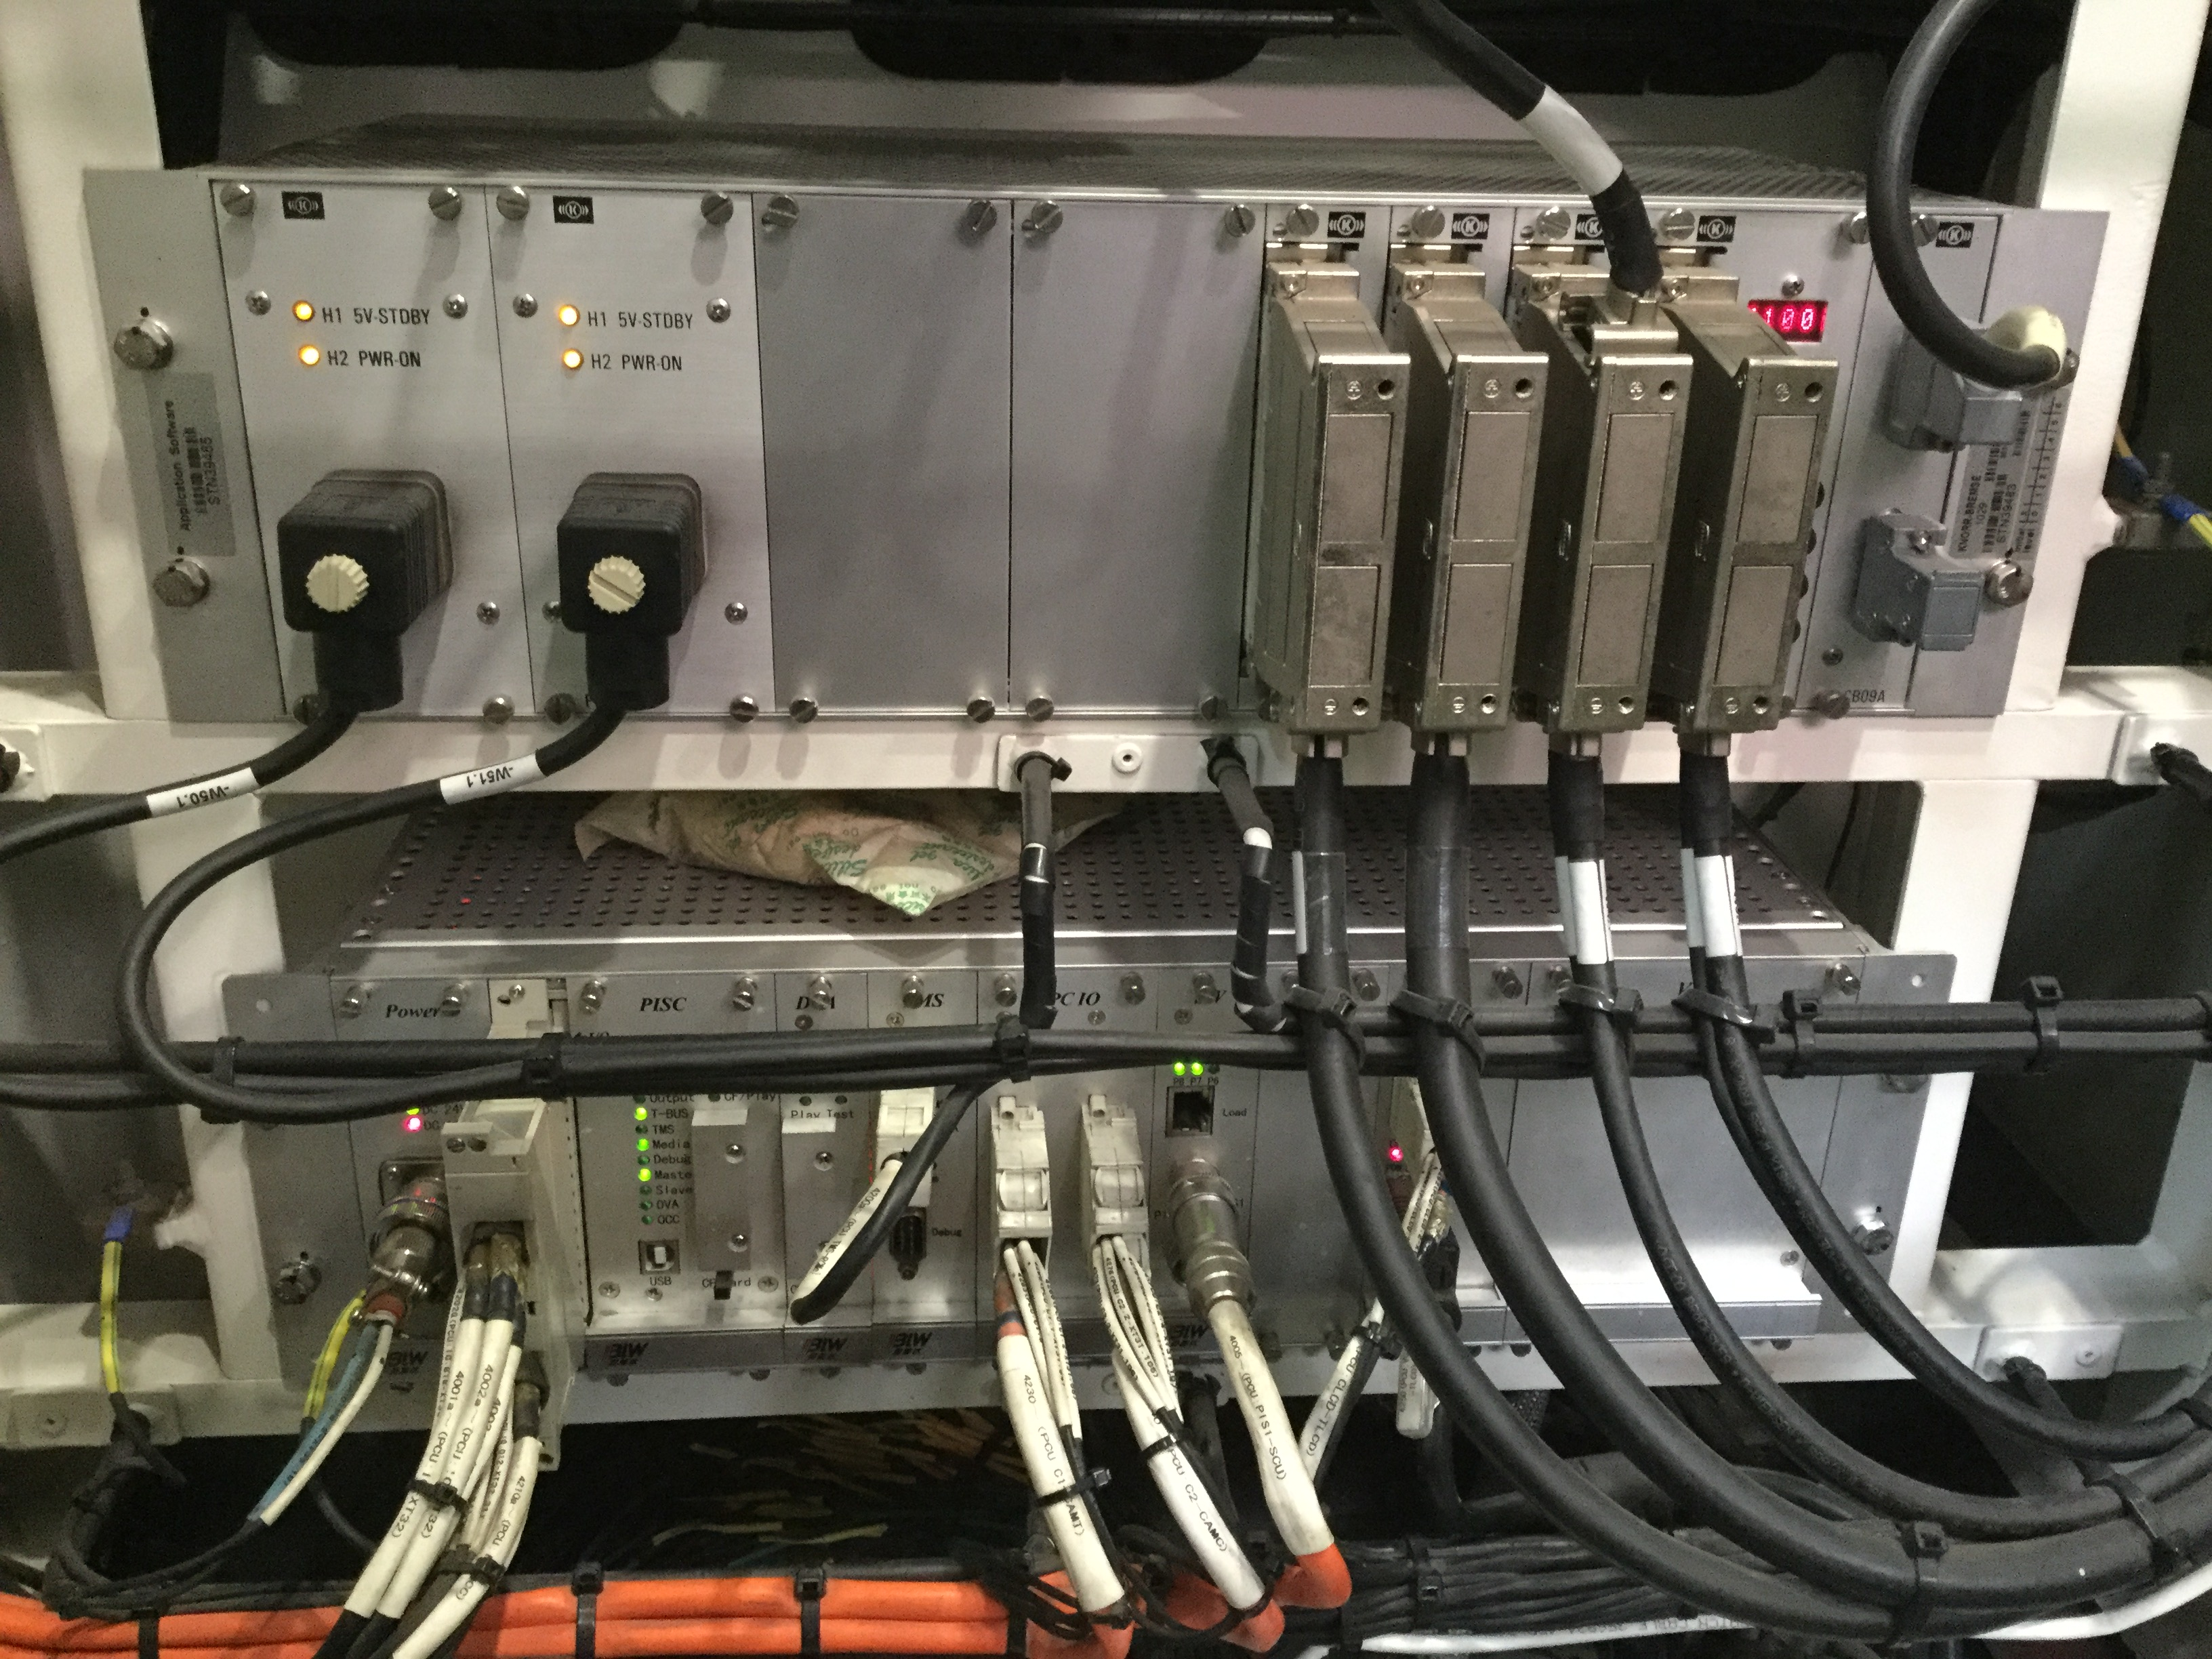
\includegraphics[width=0.75\textwidth]{./Figures/rackPIDS1.JPG}
	\caption{Fotografía de las unidades de rack del sistema PIDS en el rack de salón.}
	\label{fig:rackPIDS1}
\end{figure}


Las formaciones existentes de SOFSE fueron adquiridas durante los años 2013-2014. Si bien se observa que las redes RS485 son parte fundamental de la red TCN en estas formaciones, existe una nueva generación de redes TCN basadas en redes \textit{Ethernet} que se comenzó a especificar a partir del año 2008 por la IEC y que se expuso en demostraciones de performance recién a mediados de 2015. En el nuevo estándar de TCN basado en redes \textit{Ethernet} de tiempo real, se definen los análogos a los buses WTB y MVB, los buses ETB (\textit{Ethernet Train Backbone}) y ECN (\textit{Ethernet Consist Network}). Las empresas Siemens, Bombardier, Alstom, Mitsubishi y el Instituto Zhuzhou formaron parte del desarrollo de los nuevos estándares, saliendo al mercado entre los años 2014-2015. En comparación con la versión WTB/MVB, ETB/ECN soporta datos multimedia incluyendo video. Así, en esta nueva generación de TCN \textit{Ethernet}, tanto el CCTV como el PIDS están especificados dentro de las normas IEC62580-2 y IEC62580-4, respectivamente. Sin embargo, el PIDS y el CCTV ya existían en las soluciones de mercado ofrecidas por los fabricantes, como pudimos observar en los coches de SOFSE en los que estos sistemas se basan en redes RS485, aunque no estuvieran especificados por un estándar.\\



\pagebreak
\newpage

\section{PIDS: Sistema de información visual para pasajeros}

El PIDS de Trenes Argentinos es una solución propietaria, y no está especificada en ningún estándar. Este sistema integra un circuito cerrado de cámaras de TV (CCTV), un sistema de audio (LSP), mapas de recorrido (LDMU) y carteles de matriz led (IDU). En la figura \ref{fig:diagramaPIDS} se presenta un diagrama de su arquitectura.Se puede observar un bus de datos ubicado en la parte superior, que recorre todo el largo del plano conectandose con todos los bloques. Este bus está formado por los cables 4001, 4002 y 4003, formando una red RS485 a la que se conectan distintos módulos conectorizados. Existen dos módulos denominados DACU y FDU, encargados del micrófono, del audio, de la comunicación con los sistemas CAM T, CAM C, TCMS, OCC y de la pantalla táctil LCD del conductor (TLCD), a través del módulo PCU. Al bus RS485 también se conecta el módulo SCU, que por su ubicación central y conexionado funciona como un \textit{hub} de dispositivos. Al SCU se conecta otro conjunto de módulos: PECU1 y PECU2 indicando referencia de los laterales del tren, cámaras CAM1 y CAM2, y cuatro arreglos serie de dispositivos entre los que se encuentran los carteles de matriz led, los mapas de recorridos y parlantes. Dos de los arreglos serie integran los bloques IDU (carteles de matriz led) y LDMU (mapas de recorrido led), y los otros dos arreglos serie integran los bloques LSP o parlantes. Se puede observar que existen dos unidades IDU: IDU1 al comenzar y IDU2 al finalizar el arreglo serie. La nomenclatura corresponde con la ubicación de los carteles de matriz led en el salón de cada coche. \\

Los módulos IDU corresponden a las unidades por las que se transmiten datos a los carteles de matriz led. En el SCU termina un conjunto de cables mediante un conector Harting IO/48 P, como se puede observar en la figura \ref{fig:rackPIDS2}. Dentro del mismo, el bus RS485 que conecta el SCU con las unidades IDU está compuesto por los cables nomenclados como 4330a (RS485A), 4330b (RS485B) y 4330c (RS485C). Este punto de conexión resulta importante porque, según lo relevado en las formaciones de SOFSE, es el punto de conexión física de los carteles de matriz led de salón.\\

\begin{figure}[htbp]
	\centering
	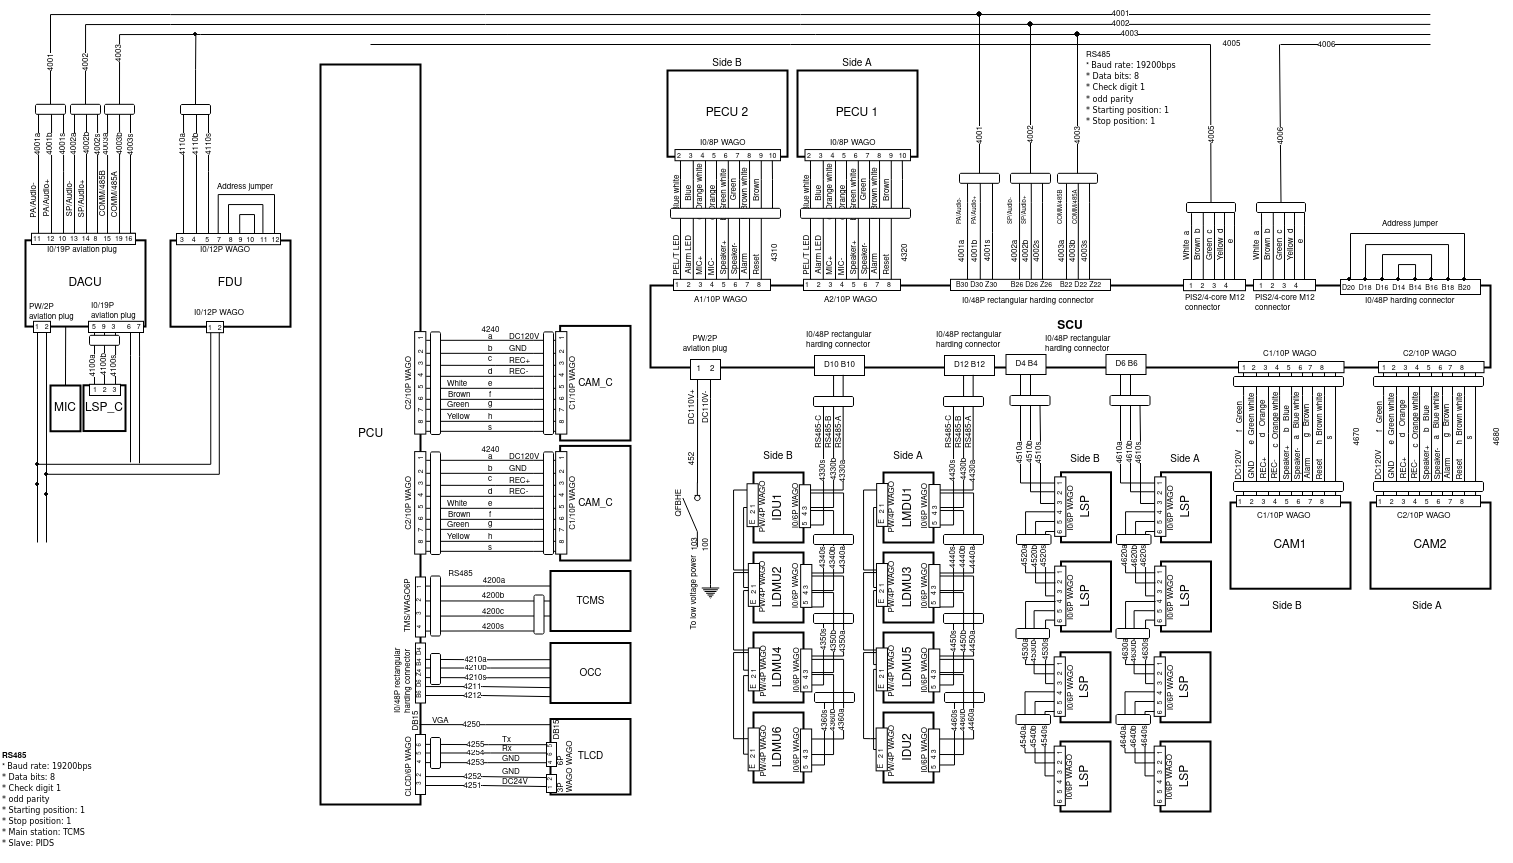
\includegraphics[width=1.66\textwidth, angle=90]{./Figures/diagramaPIDS.png}
	\caption{Diagrama de bloques del sistema PIDS, elaborado por el autor en base al plano de referencia de SOFSE.}
	\label{fig:diagramaPIDS}
\end{figure}



\begin{figure}[ht]
	\centering
	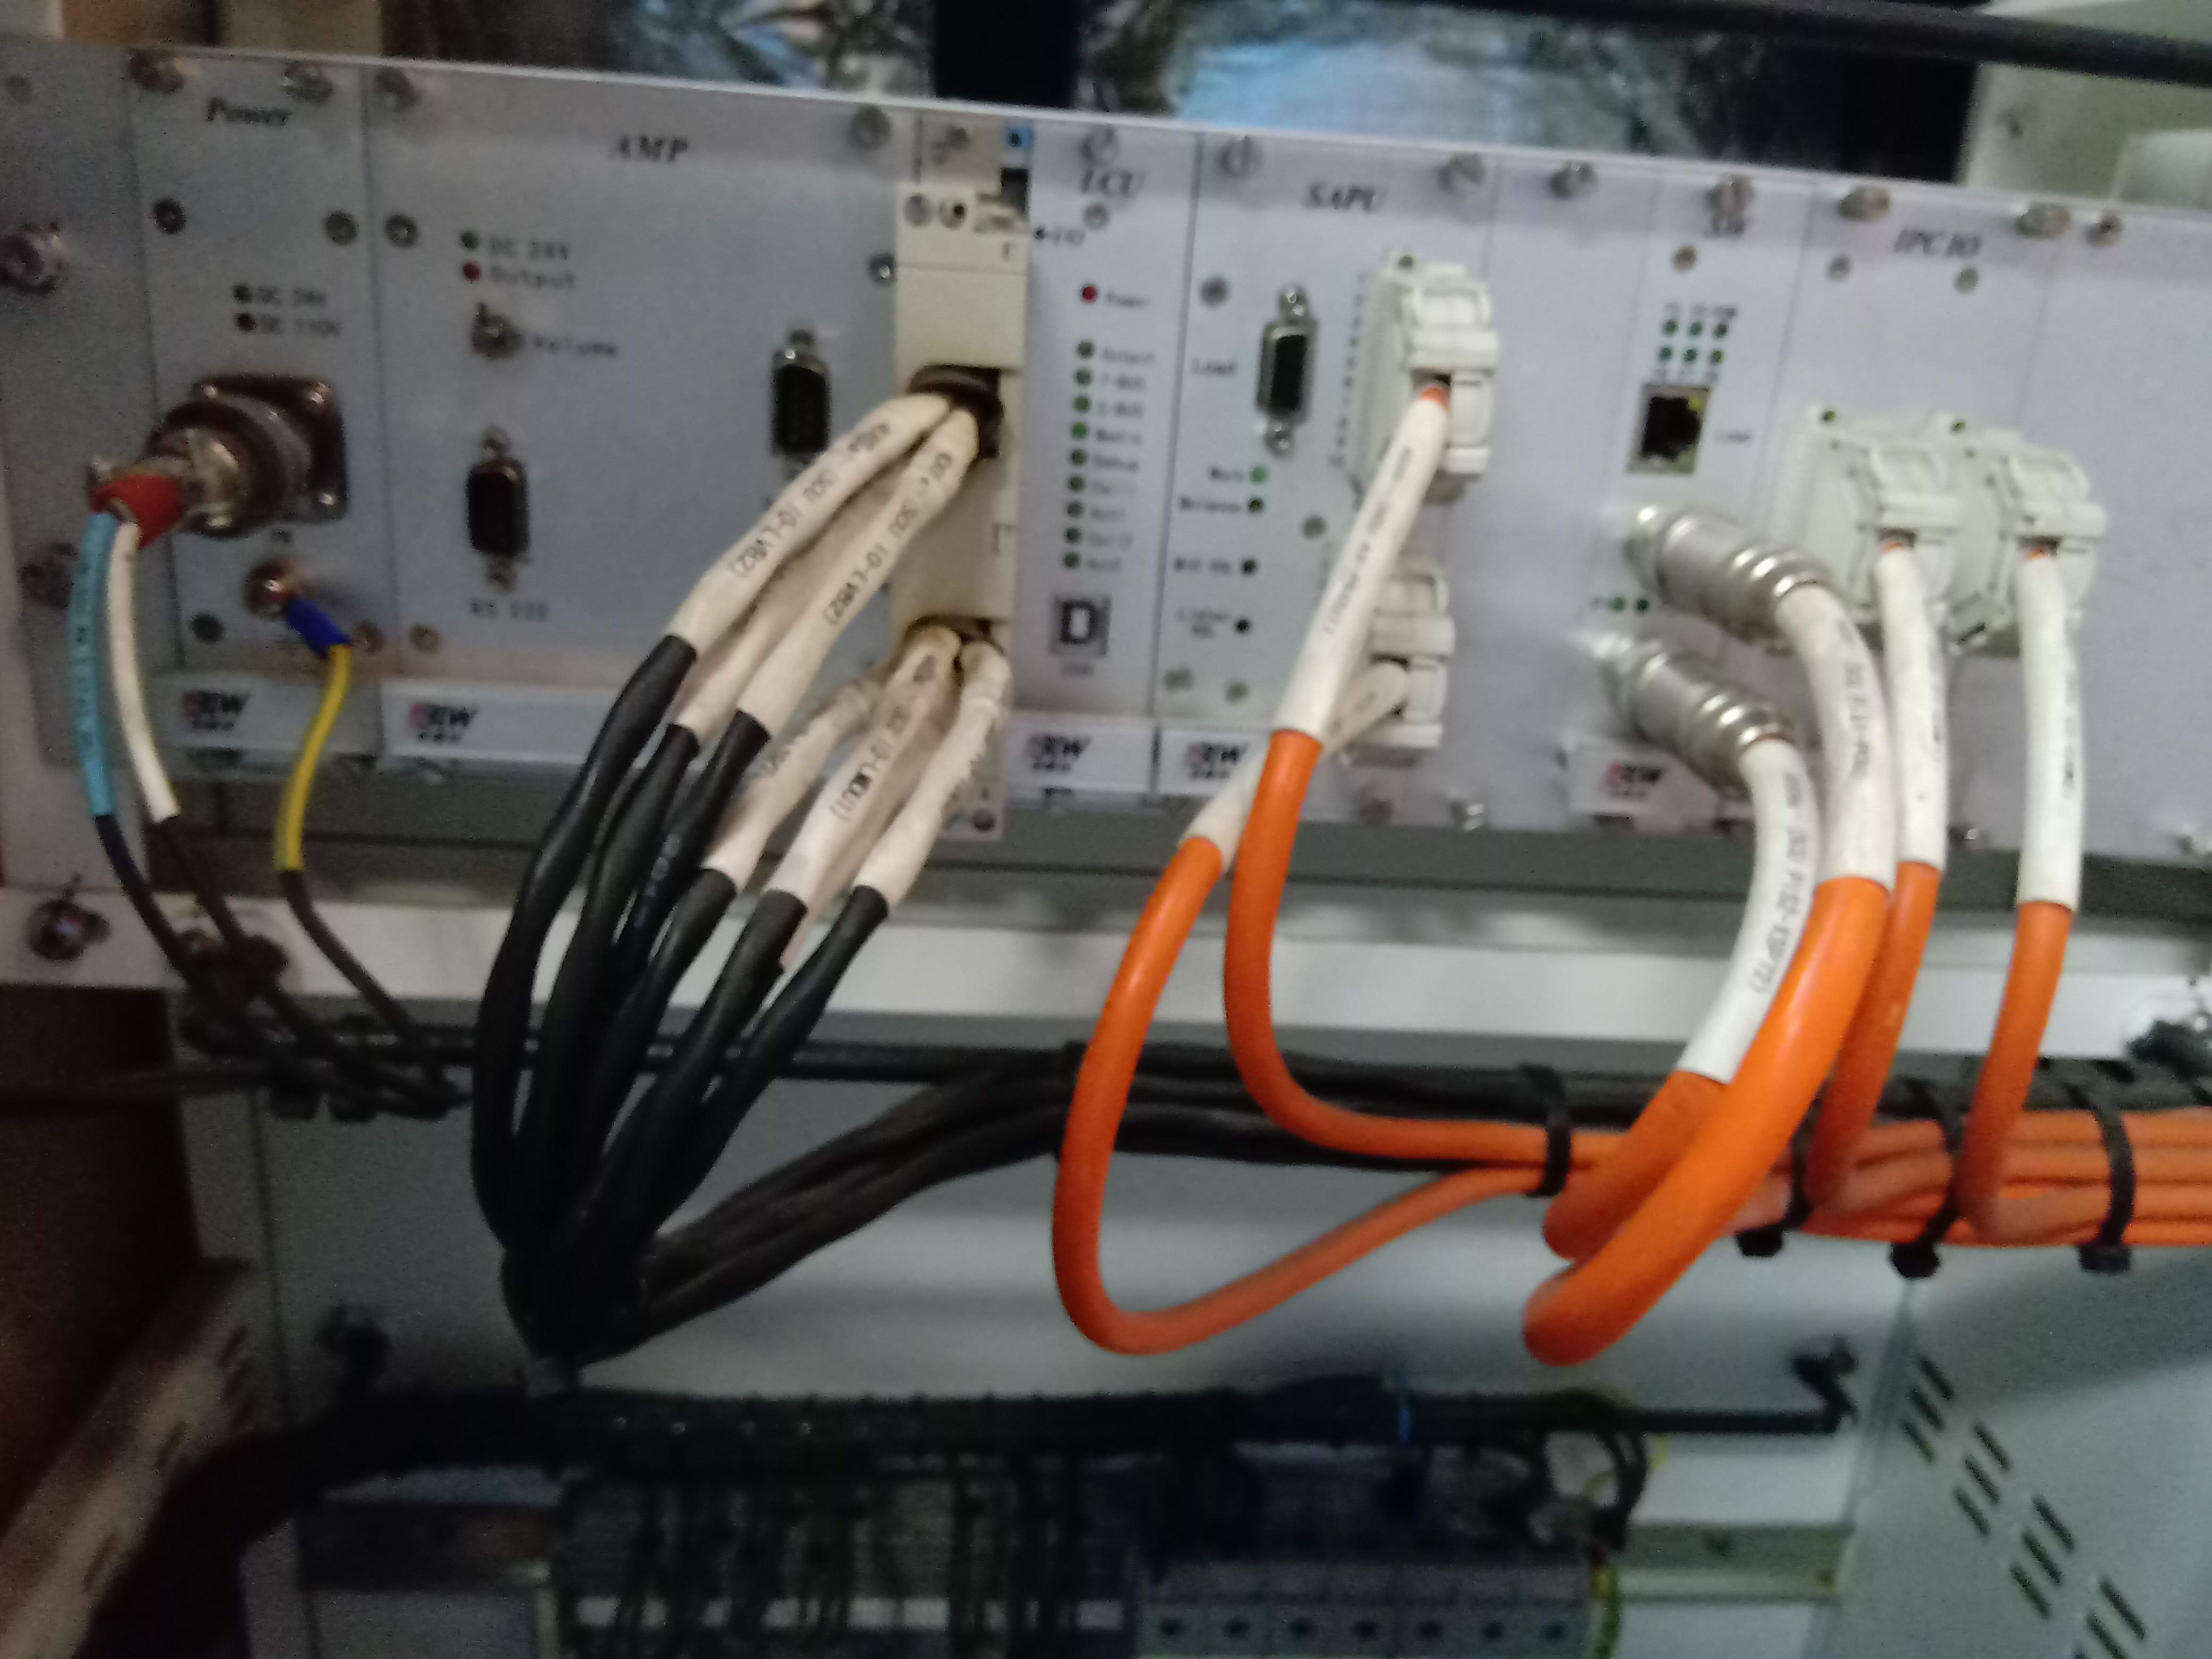
\includegraphics[width=0.75\textwidth ]{./Figures/rackPIDS2.jpg}
	\caption{Fotografía del detalle de cableado de la unidad de rack del PIDS que corresponde a los carteles LED de salón.}
	\label{fig:rackPIDS2}
\end{figure}

\section{Carteles y controladoras de matrices led}

En la sección del estado del arte de sistemas de información visual, se han presentado distintos tipos de carteles led y controladores asociados. Los carteles de matriz led de las formaciones de Trenes Argentinos están compuestos de módulos de 8x8 leds, que forman carteles de 48 módulos monocromo (rojo) para los carteles de salón y de 12 módulos bicolor (rojo-verde) de mayor tamaño para los carteles de frente y contrafrente del tren. Las placas de control de estos carteles tienen, por un lado, conexión eléctrica con la red de 110 VDC del tren, y por otro, un circuito de datos de 5 VDC que se comunica con el conjunto de chips digitales de los módulos 8x8. La figura \ref{fig:cartelIniciando} es una fotografía de un cartel de matriz led de salón inicializandose para brindar servicio al pasajero.\\

\begin{figure}[ht]
	\centering
	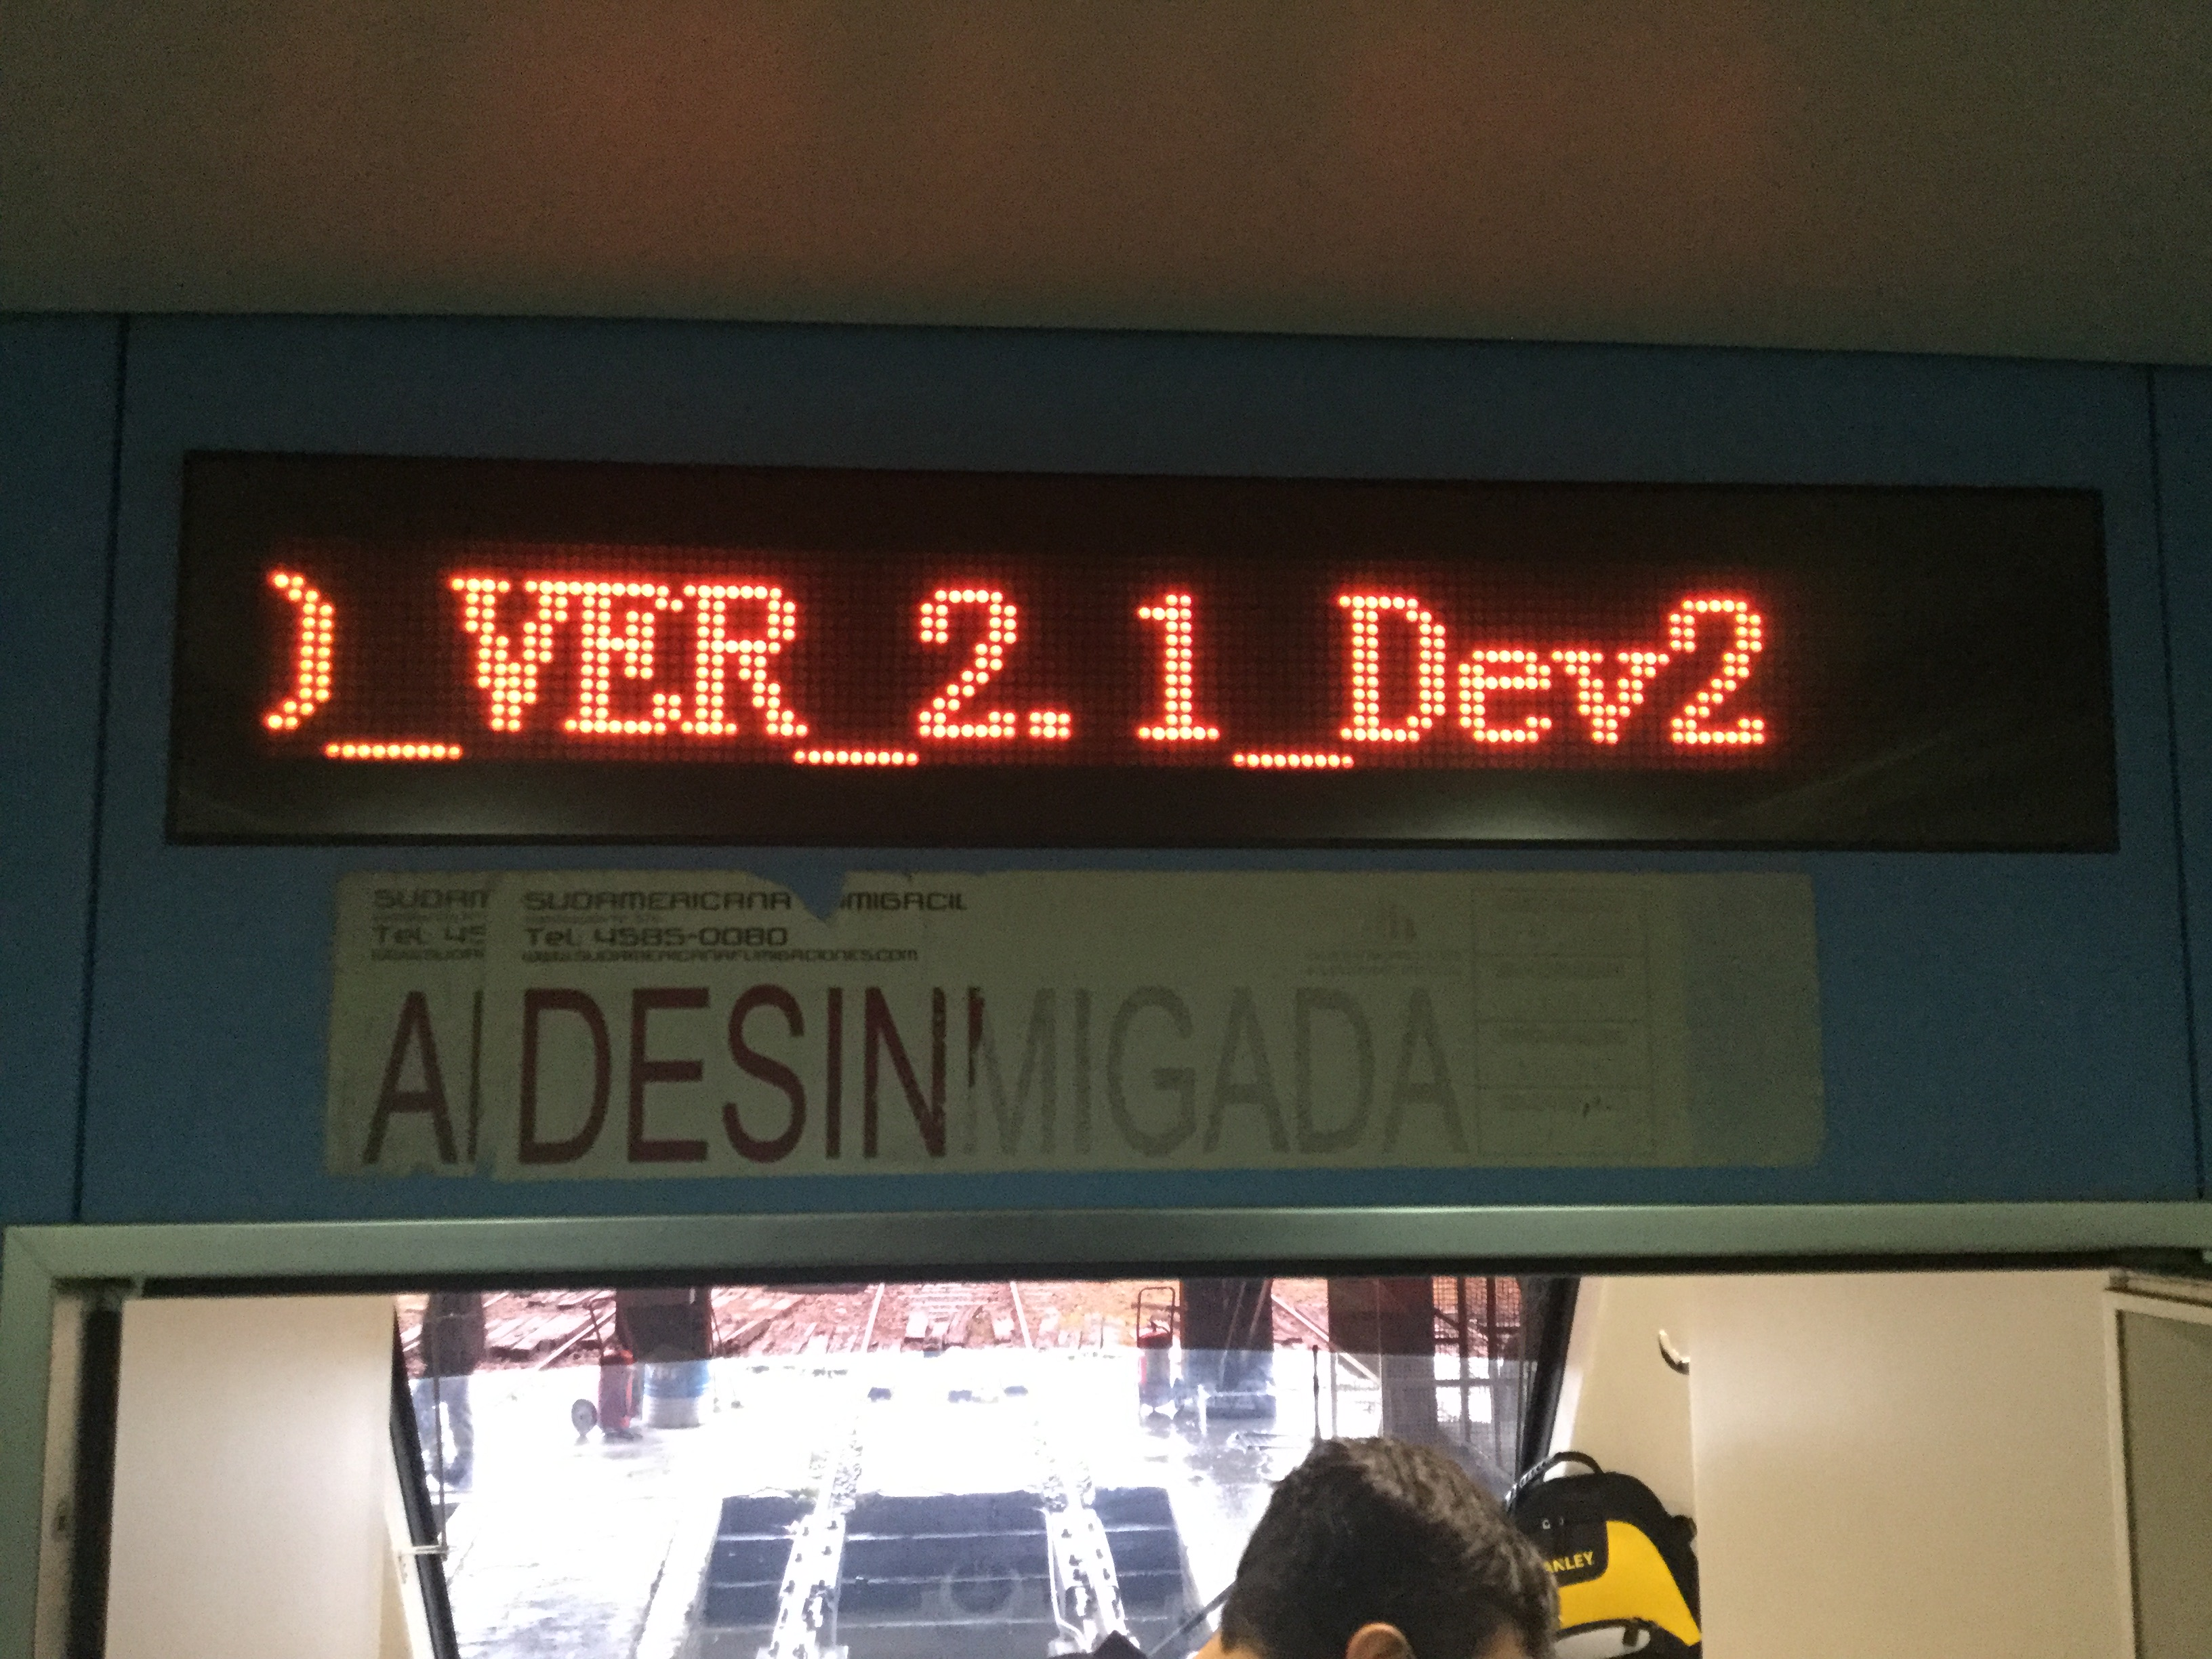
\includegraphics[width=0.75\textwidth]{./Figures/cartelIniciando.JPG}
	\caption{Fotografía de un cartel de salón inicializandose bajo una prueba de operación.}
	\label{fig:cartelIniciando}
\end{figure}
